\documentclass[journal]{IEEEtran}
\usepackage{amsmath,amssymb,amsfonts}
\usepackage{bm}
\usepackage{graphicx}
\usepackage{cite}
\graphicspath{{figs/}{../figs/}}
\hyphenation{con-ti-nu-ous ap-er-ture dis-cret-iz-ation Cram-er-Rao}

% Tighter spacing around floats and displays, within the range used by
% IEEE letters; the letter is typeset to exactly five pages without
% cutting technical content.
\setlength{\textfloatsep}{1pt plus 1pt minus 1pt}
\setlength{\floatsep}{1pt plus 1pt minus 1pt}
\setlength{\intextsep}{1pt plus 1pt minus 1pt}
\setlength{\abovecaptionskip}{2pt}
\setlength{\belowcaptionskip}{0pt}
\setlength{\abovedisplayskip}{5pt plus 2pt minus 2pt}
\setlength{\belowdisplayskip}{5pt plus 2pt minus 2pt}

\usepackage{placeins}
\usepackage[hidelinks]{hyperref}
\hypersetup{pdftitle={Range Errors as Uniform Phase Rotations in Continuous Aperture Arrays: Consequences for Near-Field Channel Estimation},pdfauthor={Yijie Zhao}}
\begin{document}

\title{Range Errors as Uniform Phase Rotations in Continuous Aperture Arrays: Consequences for Near-Field Channel Estimation}

% ---------------------------------------------------------------
%  Author block. IEEE WCL asks for member grades where applicable, an
%  explicit corresponding author, and the funding acknowledgement. The
%  received date is inserted by IEEE at production and is omitted here.
% ---------------------------------------------------------------
\author{Yijie~Zhao%
\thanks{The author is with Xidian University, Xi'an, Shaanxi 710071, China (e-mail: 25019100396@stu.xidian.edu.cn).}%
\thanks{ORCID: 0009-0007-9222-3234.}%
}

\maketitle

\begin{abstract}
Continuous aperture arrays make the near-field channel high-dimensional, although two geometric parameters govern it. A range error is a uniform phase rotation, so raw NMSE is dominated by an unidentifiable nuisance term, and estimators must be scored after a gain fit. A dictionary with a free per-atom coefficient is range-blind. A soft-argmax classifier with complex-gain fitting recovers $(r,\theta)$ and, once amplitude-calibrated, lowers NMSE by $20.9$~dB relative to LS and improves range RMSE $14\times$ relative to a refined dictionary. One further path $30$~dB down costs $49\%$ of the range accuracy.
\end{abstract}

\begin{IEEEkeywords}
6G, channel estimation, continuous aperture array (CAPA), deep learning, near-field communications.
\end{IEEEkeywords}

% ============================================================
\section{Introduction}
\IEEEPARstart{S}{ixth}-generation (6G) networks are expected to be limited by spatial degrees of freedom (DoF) rather than transmit power \cite{foschini}. The DoF of a discrete array are set by element spacing and mutual coupling, which has motivated the \emph{continuous aperture array} (CAPA): a continuous surface carrying a continuous excitation \cite{capa2024,holographic}. CAPA beamforming \cite{capaMIMO,capaOptimal}, aperture DoF \cite{capaDoF,capaOrientation,dofHolo,dofNF}, and ISAC \cite{capaISAC} have since been studied. Channel estimation for a continuous aperture appears in the holographic-MIMO lineage \cite{hmimoDFT,hmimoAngle}, there with far-field dictionaries and no identifiability analysis. The estimators developed here return the physical pair $(r,\theta)$, which transfers across discretizations for about $1$~dB (Section~IV-E). \textbf{We assume throughout a single user, a single line-of-sight path, a one-dimensional aperture, ideal orthogonal pilots, and an amplitude calibrated to within a few percent.}

All of these directions rely on accurate aperture-domain channel state information (CSI). Representing a continuous excitation takes several hundred coefficients per user, but in the near field the channel itself is fixed by two parameters, the range $r_k$ and the angle $\theta_k$. Dictionary-based compressed sensing discretizes the $(r,\theta)$ plane into a polar-domain dictionary \cite{elaa,cuidai,weidai,omp,polar,sparse,extrap}. Grid mismatch then appears, and refining the grid cannot remove it because the dictionary grows without bound.

This letter reports three findings on estimator design and evaluation, and one limitation.


\begin{enumerate}
\setcounter{enumi}{0}
\setlength{\itemsep}{1pt plus 1pt minus 1pt}
\setlength{\parsep}{0pt}
\item \textbf{The channel NMSE metric is misleading.} A range error shifts the reconstructed phase by $-2\pi\Delta r/\lambda$ \emph{uniformly} across the aperture, because $\partial d_k(s)/\partial r_k \approx 1$ for $|s| \ll r_k$. Raw NMSE is therefore dominated by this nuisance term and saturates near $2$ however well the parameters are estimated. A least-squares complex-gain fit removes it.
\item \textbf{Direct regression on the reconstruction loss is infeasible.} A range shift of $\lambda/2$ rotates the channel by $\pi$, so the manifold closes every $\lambda/2$ \emph{modulo the unknown gain}. That loss, which does not fit the gain, has period $\lambda$ and about $130$ local minima over $13$~m; descent collapses to a constant boundary output. Soft-argmax classification over the parameter grid avoids both this failure and the grid mismatch.
\item \textbf{A polar-domain dictionary with a free per-atom coefficient is range-blind.} The range derivative is collinear with the unknown complex gain to about one part in $10^{6}$, so the likelihood is almost flat in range. The fitted coefficient discards the amplitude cue, and refining the grid three times finer than $\lambda/2$ leaves the range RMSE unchanged, at the level of the nuisance-gain bound. Exploiting the calibrated amplitude instead reduces the range RMSE $14$-fold at $10$~dB, transferring without retraining.
  \item \textbf{The single-path assumption is the binding constraint.} A second path at $30$~dB SIR carries $0.1\%$ of the power, below the noise at $20$~dB SNR, and still costs $49\%$ of the range accuracy: it is coherent across the aperture, and averaging does not suppress it. Even eight times the training budget recovers at most $2\%$ \emph{at this $30$~dB operating point} (Section~S24). The estimator is therefore claimed only under the single-path model of Section~II; Section~V states this boundary explicitly.
\end{enumerate}

\noindent\textit{Notation:} $(\cdot)^{T}$ and $(\cdot)^{H}$ denote transpose and conjugate transpose, $\|\cdot\|$ the Euclidean norm, and $\jmath \triangleq \sqrt{-1}$.

% ============================================================
\section{System Model}

\subsection{CAPA Near-Field Channel}

A one-dimensional aperture of length $D$ serves $K$ single-antenna users, with aperture coordinate $s \in \mathcal{S} \triangleq [-D/2,\,D/2]$. The excitation satisfies $\int_{\mathcal{S}} |x(s)|^{2} \mathrm{d}s \leq P_{\max}$; in simulation the gain is unity, so neither this nor the pilot power $P_p$ enters the reported SNR. Users lie in the radiative near field, within the Rayleigh distance $d_{\mathrm{Rayl}} = 2D^{2}/\lambda$, and user $k$ has polar coordinates $(r_k, \theta_k)$ relative to the aperture center (Fig.~\ref{fig:geom}). The distance from aperture point $s$ to user $k$ is
\begin{equation}
d_k(s) = \sqrt{\, r_k^{2} + s^{2} - 2\, r_k\, s \sin\theta_k \,},
\end{equation}
and the spherical-wave response is
\begin{equation}
h_k(s) = \alpha_k\, \varphi_k(s),\quad \varphi_k(s) = \frac{1}{d_k(s)} \exp\!\left( -\jmath \frac{2\pi}{\lambda} d_k(s) \right),
\label{eq:chan}
\end{equation}
where the unknown complex gain $\alpha_k \triangleq |\alpha_k| e^{\jmath\psi_k}$ lumps transmit power, path loss and carrier phase, and $\varphi_k$ is the geometry-only response. We write $\varphi_k(s)$ for the continuous response and $\bm{\phi}(r_k,\theta_k) \in \mathbb{C}^{M}$ for its sampled vector; they denote the same object. The far-field plane-wave model makes $\varphi_k$ independent of $r_k$. For a near-field source it depends on both $r_k$ and $\theta_k$, and its magnitude varies across the aperture.

\begin{figure}[t]
\centering
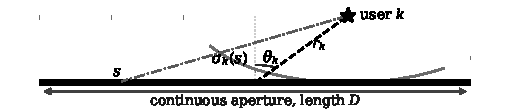
\includegraphics[width=\columnwidth]{fig0-geometry}
\caption{Near-field geometry: aperture coordinate $s$, user $k$ at $(r_k,\theta_k)$, distance $d_k(s)$, and the tangent wavefront (grey).}
\label{fig:geom}
\end{figure}

\subsection{Discretization and Observation}

Sampling at $M$ uniformly spaced points yields $\mathbf{h}_k \in \mathbb{C}^{M}$ with entries $h_k(s_m)$. Because the aperture is continuous, $M$ is a \emph{design parameter} that we may choose freely; the same aperture can be sampled at any density. With orthogonal pilots of power $P_p$, the observation after de-multiplexing is
\begin{equation}
\mathbf{y}_k = \mathbf{h}_k + \mathbf{n}_k, \qquad \mathbf{n}_k \sim \mathcal{CN}\!\left(\mathbf{0}, \sigma^{2} \mathbf{I}_M\right),
\label{eq:obs}
\end{equation}
and the per-element signal-to-noise ratio is $\mathrm{SNR} = \mathbb{E}[|h_k(s)|^{2}]/\sigma^{2}$. The complex gain is unity in simulation, so the SNR is per aperture sample and independent of the link budget. The least-squares estimate is $\widehat{\mathbf{h}}_k^{\mathrm{LS}} = \mathbf{y}_k$ with $\mathrm{NMSE}_{\mathrm{LS}} = 1/\mathrm{SNR}$, independently of $M$.

\subsection{Parametric Structure and the Nuisance Gain}

The channel \eqref{eq:chan} is fully determined by $(r_k, \theta_k)$ together with the complex gain $\alpha_k$:
\begin{equation}
\mathbf{h}_k = \alpha_k\, \bm{\phi}\!\left(r_k, \theta_k\right),
\label{eq:param}
\end{equation}
so $\mathbf{H}$ carries $4K$ real degrees of freedom ($2K$ geometric, $2K$ gain) irrespective of $M$. One property of \eqref{eq:param} is central to evaluation. Differentiating the distance term,
\begin{equation}
\frac{\partial d_k(s)}{\partial r_k} = \frac{r_k - s\sin\theta_k}{d_k(s)} = 1 + \mathcal{O}\!\left(\frac{s^{2}}{r_k^{2}}\right),
\label{eq:deriv}
\end{equation}
because $|s| \leq D/2 \ll r_k$ in every practical near-field deployment. To first order, a range error $\Delta r_k$ therefore perturbs the distance \emph{uniformly} across the aperture, and the reconstructed channel is rotated by a common phase:
\begin{equation}
\bm{\phi}(r_k + \Delta r_k, \theta_k) \;\approx\; e^{-\jmath 2\pi \Delta r_k/\lambda}\, \bm{\phi}(r_k, \theta_k).
\label{eq:commonphase}
\end{equation}

Scoring $\widehat{\mathbf{h}} = \bm{\phi}(\hat r_k, \hat\theta_k)$ by raw NMSE against $\mathbf{h}_k$ gives, by \eqref{eq:commonphase},
\begin{equation}
\mathrm{NMSE} \;\approx\; 2\left(1 - \cos\!\left(\frac{2\pi \Delta r_k}{\lambda}\right)\right),
\label{eq:nmseosc}
\end{equation}
which oscillates with period $\lambda$ and averages $2$ over a uniformly distributed range error. Raw NMSE scores an \emph{unidentifiable} nuisance phase, and says little about the geometric estimate. Since $\lambda = 0.1$~m here, reaching the LS baseline would require sub-centimetre range accuracy. It is attainable only with a known gain ($2.2\times10^{-4}$~m), and elusive otherwise ($2.4$~m). The curvature is the only unambiguous range cue, consistent with the near-field Fisher information \cite{crb,crbnf}.

Equation \eqref{eq:commonphase} has a sharper consequence. Since \eqref{eq:deriv} holds at \emph{every} aperture point, the range derivative is nearly parallel to the unknown gain. Let $c$ be their normalized inner product; it deviates from unity by $5\times10^{-7}$ at $(6~\mathrm{m},0.2)$ and $1.0\times10^{-8}$ at $(16~\mathrm{m},0.2)$. The first-order term of $\partial d/\partial r$ cancels exactly, giving $1-c\approx\cos^4\theta\,D^4/(1440r^4)$. This $r^{-4}$ law matches the measurements to a median of $2.4\%$ (Section~S21). The Fisher matrix for $(r, \theta, \Re\alpha, \Im\alpha)$ is ill conditioned, with condition number rising from $2\times10^{9}$ at broadside $5$~m to $10^{13}$ near the truncation angle. \emph{Under a free complex gain the range is only weakly identifiable}: projecting the gain subspace out leaves a range direction of residual norm $3.7\times10^{-4}$ of the original, and the RMS-averaged bound is $2.4$~m at $10$~dB, about $63\%$ of the prior standard deviation of $r$.

Three gain assumptions matter. With the gain known the bound is $2.2\times10^{-4}$~m; with it entirely unknown, $2.4$~m. Neither matches the model used here, in which $|\alpha_k|$ is known to within a few percent and the phase is unknown. A $1\%$ amplitude error costs $17\%$ at $10$~dB and $85\%$ at $20$~dB; a half-radian phase error costs under $1\%$ (Fig.~\ref{fig:calib}, Section~S14). Eliminating that phase gives $0.168$ and $0.053$~m at $10$ and $20$~dB, against measured $0.175$ and $0.077$~m, within $1.04$--$1.45$ of the bound. The bound constrains unbiased estimators; ours is biased, so its MSE may fall below it. It is a reference scale, not an optimality claim. (RMS over users with $|\theta| \le 1.2$~rad; the angle CRB diverges at endfire.) A maximum-likelihood check from truth returns a range RMSE of $0.59$~m, against $5.7$~m from random initialization. The measured angle RMSE ($4.36\times10^{-3}$~rad) lies $3.9\times$ above its bound of $1.12\times10^{-3}$~rad under the same gain assumption (Section~S3), as expected for a biased, grid-parameterized estimator.

Range information resides in two places: the absolute amplitude, which needs a calibrated link budget, and the common phase, which needs a known gain. Section~IV separates them experimentally.

The remedy is to fit the complex gain by least squares. We estimate $\alpha_k \triangleq \langle \bm{\phi}(\hat r_k,\hat\theta_k), \mathbf{y}_k\rangle / \|\bm{\phi}(\hat r_k,\hat\theta_k)\|^{2}$ from the observation and reconstruct the channel as
\begin{equation}
\widehat{\mathbf{h}}_k^{\mathrm{fit}} = \alpha_k \, \bm{\phi}\!\left(\hat r_k, \hat\theta_k\right),
\label{eq:fit}
\end{equation}
which absorbs the common phase and the amplitude. This fit gives fair NMSE scoring. The calibrated amplitude enters separately, as an input cue for range estimation. After the fit, only the wavefront \emph{shape} carries parameter information: an angle error tilts the phase, and a range error perturbs it quadratically by $\mathcal{O}(s^{2}/r_k^{2})$ per \eqref{eq:deriv}. The reconstruction \eqref{eq:fit} is confined to at most four real dimensions per user; the LS estimate ranges over all of $\mathbb{C}^{M}$.
% ============================================================
\section{Proposed Deep Parametric Estimator}

\subsection{Why Direct Regression Fails}

Near-field Fisher/CRB structure is known for source localization and discrete arrays \cite{crb,crbnf}. We state it for a \emph{continuous} aperture, give the closed-form degeneracy law, and build the evaluation pipeline it implies. Learning-based estimators are established for conventional MIMO \cite{dlceFound,mdlFound,dlce}. A natural design regresses $(r_k, \theta_k)$ on the reconstruction loss. This fails. By \eqref{eq:nmseosc} that loss oscillates with period $\lambda$ in $\hat r_k$, since a shift of $\lambda/2$ rotates the channel by $\pi$ and admits about $130$ local minima. The network collapses to $\hat r_k = 5$~m (holdout range RMSE $7.59$~m).

The collapse is structural and dictates the estimator architecture.

\subsection{Classification with Soft-Argmax Decoding}

We treat estimation as classification \cite{softargmax}. Let $\{c^{(r)}_i\}_{i=1}^{G_r}$ and $\{c^{(\theta)}_j\}_{j=1}^{G_\theta}$ be uniform grids over range and angle. With $G_r=128$ the range spacing is about $0.102$~m, comparable to the oscillation period $\lambda$. The soft-argmax sub-bin interpolation makes this adequate, as the ablations confirm. A shared trunk produces two logit vectors, and the estimate is the soft-argmax of the corresponding posteriors:
\begin{equation}
\begin{aligned}
\hat r_k &= \sum_{i=1}^{G_r} \mathrm{softmax}\!\left(\mathbf{z}^{(r)}/\tau\right)_{i} c^{(r)}_i, \\
\hat\theta_k &= \sum_{j=1}^{G_\theta} \mathrm{softmax}\!\left(\mathbf{z}^{(\theta)}/\tau\right)_{j} c^{(\theta)}_j,
\end{aligned}
\label{eq:softargmax}
\end{equation}
where $\tau$ is a decoding temperature. Training uses a cross-entropy loss against soft labels, i.e.,\ Gaussian kernels of width $\sigma_r$ and $\sigma_\theta$ centered on the true parameter values. These labels give smooth gradients and sub-bin supervision.

Three properties support this choice. Cross-entropy is smooth, unlike the oscillating loss. The soft-argmax of \eqref{eq:softargmax} interpolates between bin centers, so the estimate is continuous and free of grid mismatch; the grid merely parameterizes the output distribution. Since the grid is over physical parameters, the output is independent of $M$ by construction.

\subsection{Complex-Gain Fitting and Full Pipeline}

The complete estimator is: (i) preprocess $\mathbf{y}_k$; (ii) obtain $(\hat r_k, \hat\theta_k)$ from \eqref{eq:softargmax}; (iii) fit the complex gain and reconstruct by \eqref{eq:fit}. Step (iii) makes the geometric estimate usable (Section~II-C).

We use the raw real and imaginary parts of the observation, rescaled by a fixed constant. We also evaluated one structure-aware alternative, the phase-differenced representation $\mathbf{y}_k/y_k(s_{M/2})$ with the normalized magnitude profile (the \emph{magnitude-normalized} variant), which retains the wavefront phase but removes the absolute amplitude. The raw representation gave the best range accuracy. The scale of $|h_k(s)| \propto 1/r_k$ is itself a monotone range cue, and normalizing it away discards information.

\subsection{Complexity}

The trunk has hidden sizes $N_1,N_2,N_3$, giving $\mathcal{O}(M N_1 + N_1N_2 + N_2N_3)$ inference cost, and the soft-argmax adds $\mathcal{O}(G_r + G_\theta)$. Polar-domain compressed sensing with $G$ atoms costs $\mathcal{O}(MKG)$ per sample, plus $\mathcal{O}(MKG_{\mathrm{ref}})$ per refinement round. Measured inference times for $M=256$ over $1200$ samples are $2.6$~ms (LS), $765$~ms (LMMSE), $76$~ms (OMP $50\times100$), $86.1$~s (OMP with coarse-to-fine refinement) and \textbf{$24.6$~ms} (proposed).

% ============================================================
\section{Simulation Results}

\subsection{Setup}

Training uses $10^{6}$ \emph{noiseless} channels from a $2\times10^{6}$ dataset (seed $0$). Noise is injected on the fly at a uniformly drawn SNR in $[-5,20]$~dB. All training and inference run on a commodity CPU without a GPU. Results use an independent holdout (seed $999999$), unused in training or selection. Baselines are LS, LMMSE, and L2-normalized polar-grid dictionary matching on $50\times100$ and $100\times200$ grids, with and without refinement (Section~S10). LMMSE is a channel estimator, so the gain-fitted NMSE compares reconstruction, not parameter estimation. It uses the \emph{sample covariance of the evaluation set}, a genie-aided oracle stronger than any practical LMMSE, so the comparison is conservative.

The supplementary material states the configuration verbatim (Sections~S10, S19): a $3$~GHz carrier over a $1$~m aperture, $M=256$ unless stated, users uniform in $r\in[5,18]$~m and $\theta\in[-\pi/2,\pi/2]$ (Rayleigh $20$~m), and a $1024$--$512$--$256$ trunk ($1.28\times10^{6}$ parameters) trained for $4000$ steps at batch $2048$. Both ablations of Section~IV-D share that budget, so Section~IV-D and~IV-F compare at equal effort.

\subsection{The Metric Artifact}

Table~\ref{tab:metric} isolates the effect identified in Section~II-C. Scored by raw NMSE, every parametric method looks severely misleading: the proposed estimator reaches 1.99, LS $0.10$, LMMSE $0.0092$. After the least-squares gain fit of \eqref{eq:fit} the ordering reverses. The proposed estimator reaches $0.81\times10^{-3}$, beating LS by $20.9$~dB and LMMSE by $10.6$~dB. LS and LMMSE are unaffected, because they estimate the channel directly.

\begin{table}[t]
\centering
\caption{Nuisance-gain fit and range accuracy, SNR $=10$~dB, $M=256$. The NMSE columns expose the artifact and coincide for LS, LMMSE and DL, whose gain fit \eqref{eq:fit} is undefined. $\dagger$: post hoc range (angle undefined). $\ddagger$: amplitude readout only (angle undefined). ``OMP + refinement'': coarse-to-fine dictionary refinement.}
\label{tab:metric}
\footnotesize
\setlength{\tabcolsep}{1.5pt}
\renewcommand{\arraystretch}{0.94}
\begin{tabular}{@{}l c c c c@{}}
\hline
\textbf{Estimator} & \textbf{NMSE} & \textbf{NMSE} & \textbf{RMSE} & \textbf{RMSE}\\
 & \textbf{raw} & \textbf{fit} & \textbf{range (m)} & \textbf{angle (rad)}\\
\hline
LS & 0.100 & 0.100 & -- & --\\
LMMSE & 0.0092 & 0.0092 & -- & --\\
DL channel est. & $4.6\times10^{-2}$ & $4.6\times10^{-2}$ & 2.53 & $1.05\times10^{-2}$\\
OMP $50\times100$ & 2.04 & $1.38\times10^{-2}$ & 2.66 & $1.02\times10^{-2}$\\
OMP $100\times200$ & 2.07 & $4.00\times10^{-3}$ & 2.49 & $6.41\times10^{-3}$\\
OMP + refinement & 2.01 & $8.43\times10^{-4}$ & 2.50 & $4.56\times10^{-3}$\\
LISTA-CP dict.$\dagger$ & -- & -- & 5.31 & --\\
OMP + amp. readout$\ddagger$ & -- & -- & 0.34 & --\\
\hline
\textbf{Proposed} & 1.99 & $0.81\times10^{-3}$ & \textbf{0.18} & \textbf{$4.36\times10^{-3}$}\\
\hline
\end{tabular}
\end{table}

Raw NMSE must not be used to compare parametric with non-parametric near-field estimators. After the nuisance gain is removed, the learned estimator is the most accurate \emph{in range}, by an order of magnitude. At $10$~dB its channel NMSE is $0.18$~dB \emph{below} the refined dictionary, its angle is better, and its runtime is $3500\times$ lower.

A deep estimator of matched size ($1.31$~M) sharpens the point. At $10$~dB its gain-fitted NMSE is $4.6\times10^{-2}$, $54\times$ worse than the refined dictionary's, yet its implied range is equally blind ($2.53$~m). A CNN of matched size gives $2.57$~m, so the range stays in $2.50$--$2.57$~m across an $84$-fold NMSE span, from $8.43\times10^{-4}$ to $7.05\times10^{-2}$. Quadrupling the budget cuts its NMSE to $1.9\times10^{-3}$, within $2.4\times$ of ours, and leaves the range at $2.01$~m. At $20$~dB a better NMSE yields a \emph{worse} range. NMSE therefore does not order range accuracy. On \emph{noise-free} data the dictionary still returns $0.76$~m, so the flatness is not a noise-fitting artifact. The information is nevertheless \emph{inside} the network: a probe on the frozen features of the $4\times$-budget CNN reaches $0.19$~m, within $7\%$ of ours, while its output implies $2.05$~m (Sections~S11--S13).
\subsection{Range Ambiguity of Dictionary Methods}

Table~\ref{tab:metric} exposes a second limitation. At $10$~dB the three dictionary baselines return $2.49$--$2.66$~m, independent of grid density, and only $1.23$--$1.61$~m at $20$~dB. Aliasing is ruled out: refining from $0.131$ to $0.016$~m, finer than $\lambda/2$, changes the RMSE by under $0.1\%$. The failure lies in the fitting, not the sampling. The coefficient absorbs the amplitude, which is where the range information resides. A minimum-residual per-atom gain fit lowers the dictionary error from $7.46$ to $3.10$~m, still above the $2.50$~m refined baseline (Section~S18). A one-line amplitude readout $\hat r = 1/\mathrm{mean}_s|y(s)|$ restores $0.34$~m.

Multipath at $30$~dB SIR costs $49\%$ of the range accuracy, and retraining recovers only $2\%$ at that operating point (Section~S24). A Rician channel at $K=10$~dB costs $15\times$, and a co-pilot behaves as a second path (Section~S23). The deeper reason is the degeneracy of Section~II-C: atoms for different $r$ differ almost entirely by a common phase, so once the coefficient is fitted the likelihood is nearly flat. The proposed estimator does better ($0.18$~m) by exploiting the \emph{absolute} amplitude. That cue alone accounts for $76\%$ of the improvement in dB, and learning adds $1.9\times$.

The proposed estimator attains the lowest gain-fitted NMSE of any row; the $0.18$~dB margin over the refined dictionary is within the three-seed $95\%$ interval, whereas the order-of-magnitude range gap is not. Learning the dictionary does not close the gap. An unrolled LISTA-CP of $524$k parameters at the same budget reaches $5.31$~m, worse than the plain dictionary it is meant to improve, and does not improve with SNR ($5.26$~m at $20$~dB). The refined baseline overtakes it only above $10$~dB. At $20$~dB it is $0.80$~dB lower in NMSE and $1.34\times$ lower in angle, yet $16.3\times$ worse in range. Refinement costs $86.1$~s per $1200$ samples against $24.6$~ms. That is $3500\times$ the runtime, for comparable channel accuracy and $14\times$ better range.

\subsection{Estimation Accuracy and Input Representation}

\begin{figure}[t]
\centering
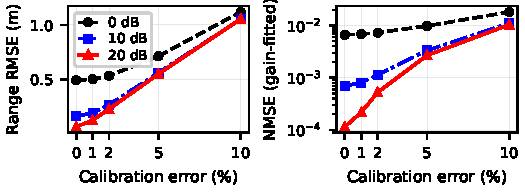
\includegraphics[width=\columnwidth]{fig5-calibration}
\caption{Range RMSE (left) and gain-fitted NMSE (right) against amplitude calibration error (three seeds). Above $3\%$ the SNR curves converge: at $10\%$ the $0$~dB and $20$~dB curves differ by $6\%$, against sevenfold at perfect calibration.}
\label{fig:calib}
\end{figure}



\begin{figure}[t]
\centering
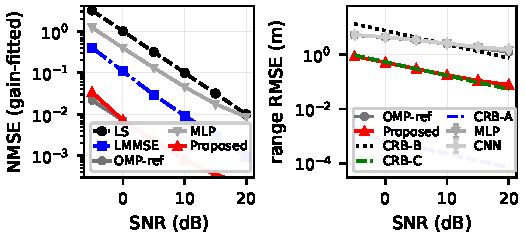
\includegraphics[width=\columnwidth]{fig1-nmse-range}
\caption{Channel NMSE after the complex-gain fit (left) and range RMSE (right) at $M=256$ (three seeds), with range Cram\'er--Rao bounds under three gain assumptions: A, gain known; B, unknown; C, phase unknown (assumed here). Deep MLP/CNN are matched-size deep channel estimators of Section~IV-B. All baselines and deep estimators lie within $12\%$ of the B curve near $10$~dB (within $5\%$ for the refined and dense grids).}
\label{fig:nmse}
\end{figure}

Fig.~\ref{fig:nmse} reports NMSE (gain-fitted) and range RMSE against SNR. The proposed estimator attains $0.81\times10^{-3}$ at $10$~dB. The margin \emph{narrows} as LS and LMMSE improve and the parametric estimator approaches its floor: the gain over LS falls from $21.4$~dB at $0$~dB SNR to $16.7$~dB at $20$~dB. The amplitude readout reaches $0.34$~m, so learning buys $1.9\times$. The raw input is best in range at every SNR. Above $10$~dB the magnitude-normalized variant attains lower NMSE. Its range, however, is $11$--$13\times$ worse, which points to the \emph{absolute} amplitude as the operative cue (Section~S16) \cite{crb,crbnf}.

The high-SNR range floor is a decoding artifact, exposed by evaluating at $40$~dB SNR. Lowering the soft-argmax temperature from $1.0$ to $0.25$ cuts the $40$~dB floor from $0.0497$ to $0.0379$~m, leaving $10$~dB unchanged (Section~S22). Replacing the classification heads by regression heads at the same budget degrades the $10$~dB NMSE from $0.81\times10^{-3}$ to $2.16\times10^{-2}$ ($26.7\times$). The loss is concentrated in the angle: range RMSE rises only from $0.18$ to $0.19$~m, but angle RMSE rises $2.7\times$. That is the signature of the oscillatory manifold of Section~III-A.

\subsection{Discretization Agnosticism}

Because the output is physical, a model trained at one discretization applies at another. Trained on $M=\!128$ and evaluated at $256$ and $512$ by linear interpolation on the real and imaginary parts separately, it pays $0.62$--$1.01$~dB against a natively trained model, about $1$~dB. Dictionary baselines must be rebuilt for every $M$. In CAPA, $M$ is a design choice rather than a physical constraint (Section~S9). A second aperture axis relieves the degeneracy without removing it (Section~S15), and atomic-norm minimization does not beat the grid dictionary it replaces (Section~S20).

\subsection{Capacity under a Fixed Compute Budget}

Fixing the budget in \emph{steps} rather than wall-clock time, three trunks of $0.48$, $1.28$ and $2.29$~M parameters give $10$~dB NMSE of $1.19\pm0.13$, $0.81\pm0.05$ and $0.76\pm0.02$ ($10^{-3}$). The smallest is worse by $47\%$, with non-overlapping intervals; the two larger trunks are $6.2\%$ apart. Capacity saturates near $1.28$~M (Section~S19).

\FloatBarrier
\section{Conclusion}

Two lessons follow. First, a range error is a uniform phase rotation, so channel NMSE must carry a complex-gain fit before parametric estimators are compared; a learned geometric estimator then beats LS and LMMSE. Second, the reconstruction loss oscillates with period $\lambda$ in range, so regression against it is infeasible, whereas soft-argmax classification is well conditioned and discretization-agnostic. Dictionaries fail for the same reason and must be rebuilt for every $M$; because the output is physical, a model trained at $M=128$ transfers to $256$ and $512$ for about $1$~dB. Accuracy is limited by calibration rather than by SNR: a $1\%$ gain error raises the $20$~dB range RMSE from $0.07$ to $0.13$~m; $5\%$ raises it to $0.55$~m (Section~S14, Fig.~\ref{fig:calib}). LoS is assumed: one extra path at $30$~dB signal-to-interference ratio costs $49\%$ (retraining recovers $2\%$ with eight times the budget), a Rician channel with $K$-factor $10$~dB costs $15\times$ the range RMSE, and a co-pilot acts as a second path (Section~S23). Users are independent: RMSE identical at $1$ and $16$ users (Section~S17.2), and a 2-D aperture relieves the degeneracy without removing it (Sections~S15, S20).

\noindent\textit{Data and code availability:} every reported number is recomputed from archived result files by the automated script in the reproduction package (Section~S25).

% ============================================================
\FloatBarrier
\begin{thebibliography}{99}
\footnotesize
\setlength{\itemsep}{0pt}
\setlength{\parskip}{0pt}
\setlength{\baselineskip}{8.3pt}

% ------------------------------------------------------------------
% BIBLIOGRAPHY: every entry re-derived from Crossref / arXiv in Oct 2026, carrying
% the publisher's author list and venue, with volume and pages where available.
% ------------------------------------------------------------------

\bibitem{foschini}
G. J. Foschini and M. J. Gans, "On limits of wireless communications in a fading environment when using multiple antennas," \emph{Wireless Pers. Commun.}, vol. 6, pp. 311--335, 1998.
\bibitem{capa2024}
Y. Liu, C. Ouyang, Z. Wang, J. Xu, X. Mu, and Z. Ding, "CAPA: Continuous-aperture arrays for revolutionizing 6G wireless communications," \emph{IEEE Wireless Commun.}, vol. 32, no. 4, pp. 38--45, 2025.
\bibitem{holographic}
C. Huang, S. Hu, G. C. Alexandropoulos, A. Zappone, C. Yuen, R. Zhang, M. Di Renzo, and M. Debbah, "Holographic MIMO surfaces for 6G wireless networks: Opportunities, challenges, and trends," \emph{IEEE Wireless Commun.}, vol. 27, pp. 118--125, 2020.
\bibitem{capaMIMO}
Z. Wang, C. Ouyang, and Y. Liu, "Beamforming design for continuous aperture array (CAPA)-based MIMO systems," \emph{IEEE Trans. Wireless Commun.}, vol. 25, pp. 2167--2182, 2026.
\bibitem{capaOptimal}
Z. Wang, C. Ouyang, and Y. Liu, "Optimal beamforming for multi-user continuous aperture array (CAPA) systems," \emph{IEEE Trans. Commun.}, vol. 73, no. 10, pp. 9207--9221, 2025.
\bibitem{capaDoF}
S. T. Duong and T. Le-Ngoc, "Spatial degrees of freedom in distance domain of continuous aperture for broadside case in near-field region," in \emph{Proc. IEEE GLOBECOM}, pp. 545--550, 2025.
\bibitem{capaOrientation}
Y. Guo, Y. Zhang, Z. Wang, M. Shang, Y. Chen, and Y. Liu, "Impact of array orientations on degrees of freedom for continuous aperture arrays (CAPA)," \emph{IEEE Wireless Commun. Lett.}, vol. 14, pp. 2476--2480, 2025.
\bibitem{dofHolo}
A. Pizzo, T. L. Marzetta, and L. Sanguinetti, "Degrees of freedom of holographic MIMO channels," in \emph{Proc. IEEE SPAWC}, pp. 1--5, 2020.
\bibitem{dofNF}
H. Chen, S. Yue, M. Di Renzo, and H. Zhang, "Degrees of freedom of holographic MIMO in multi-user near-field channels," \emph{IEEE Commun. Lett.}, vol. 29, pp. 1186--1190, 2025.
\bibitem{capaISAC}
B. Zhao, C. Ouyang, X. Zhang, H. Shin, and Y. Liu, "Downlink and uplink ISAC in continuous-aperture array (CAPA) systems," \emph{IEEE Trans. Wireless Commun.}, vol. 25, pp. 3592--3609, 2026.
\bibitem{hmimoDFT}
A. A. D'Amico, G. Bacci, and L. Sanguinetti, "DFT-based channel estimation for holographic MIMO," in \emph{Proc. 57th Asilomar Conf. Signals, Syst., Comput.}, pp. 353--357, 2023.
\bibitem{hmimoAngle}
Y. Chen, Y. Wang, Z. Wang, and Z. Han, "Angular-distance based channel estimation for holographic MIMO," \emph{IEEE J. Sel. Areas Commun.}, vol. 42, pp. 1684--1702, 2024.
\bibitem{elaa}
S. Ye, M. Xiao, M.-W. Kwan, Z. Ma, Y. Huang, and G. Karagiannidis, "Extremely large aperture array (ELAA) communications: Foundations, research advances and challenges," \emph{IEEE Open J. Commun. Soc.}, vol. 5, pp. 7075--7120, 2024.
\bibitem{cuidai}
M. Cui and L. Dai, "Channel estimation for extremely large-scale MIMO: Far-field or near-field?," \emph{IEEE Trans. Commun.}, vol. 70, pp. 2663--2677, 2022.
\bibitem{weidai}
X. Wei and L. Dai, "Channel estimation for extremely large-scale massive MIMO: Far-field, near-field, or hybrid-field," \emph{IEEE Commun. Lett.}, vol. 26, pp. 177--181, 2022.
\bibitem{omp}
J. A. Tropp and A. C. Gilbert, "Signal recovery from random measurements via orthogonal matching pursuit," \emph{IEEE Trans. Inform. Theory}, vol. 53, pp. 4655--4666, 2007.
\bibitem{polar}
A. Hussain, A. Abdallah, and A. M. Eltawil, "Redefining polar boundaries for near-field channel estimation for ultra-massive MIMO antenna arrays," \emph{IEEE Trans. Wireless Commun.}, vol. 24, pp. 8193--8207, 2025.
\bibitem{sparse}
V. B. Shukla and I. Atzeni, "Sparse near-field channel estimation for XL-MIMO via adaptive filtering," in \emph{Proc. WSA}, pp. 60--65, 2025.
\bibitem{extrap}
J. Lu, J. Zhang, H. Lei, H. Xiao, B. Ai, and D. W. K. Ng, "Near-field spatial-domain channel extrapolation for XL-MIMO systems," \emph{IEEE Trans. Wireless Commun.}, vol. 25, pp. 4343--4357, 2026.
\bibitem{crb}
H. Hua, J. Xu, and Y. C. Eldar, "Near-field 3D localization via MIMO radar: Cramer-Rao bound analysis and estimator design," \emph{IEEE Trans. Signal Process.}, vol. 72, pp. 3879--3895, 2024.
\bibitem{crbnf}
Y. Begriche, M. Thameri, and K. Abed-Meraim, "Exact Cramer-Rao bound for near field source localization," in \emph{Proc. ISSPA}, pp. 718--721, 2012.

\bibitem{dlceFound}
H. Ye, G. Y. Li, and B.-H. Juang, "Power of deep learning for channel estimation and signal detection in OFDM systems," \emph{IEEE Wireless Commun. Lett.}, vol. 7, pp. 114--117, 2018.
\bibitem{mdlFound}
H. He, S. Jin, and C.-K. Wen, "Model-driven deep learning for physical layer communications," \emph{IEEE Wireless Commun.}, vol. 26, pp. 77--83, 2019.
\bibitem{dlce}
Y. Gao, Q. Chen, L. He, Z. Wang, Y. Huang, and J. Zhang, "Artificial intelligence enabled joint channel estimation and signal detection for massive MIMO systems," \emph{Chinese J. Electron.}, vol. 35, pp. 178--195, 2026.
\bibitem{softargmax}
A. Nibali, Z. He, S. Morgan, and L. Prendergast, "Numerical coordinate regression with convolutional neural networks," arXiv preprint arXiv:1801.07372, 2018.
\end{thebibliography}

\end{document}